\documentclass[12pt,compress,ngerman,utf8,t]{beamer}
\usepackage[ngerman]{babel}
\usepackage{calc}
\usepackage{ragged2e,wasysym,multicol,mathtools,txfonts}
\usepackage[protrusion=true,expansion=true]{microtype}
\usepackage{booktabs}
\usepackage{multimedia}
\hypersetup{colorlinks=true}

\graphicspath{{images/}}

\title[Nullwissenbeweise]{Die wundersame Welt der \\ Nullwissenbeweise}
\author[Ingo Blechschmidt, Anna Rubeck]{\scriptsize
\vspace*{-1em} \\
\textbf{UniMentoSchule am 2. März 2018} \\
\emph{Fragen sind jederzeit willkommen! Bitte nicht bis zum Ende aufsparen.} \\
\medskip
Ingo Blechschmidt und Anna Rubeck \\
Lehrstuhl für Algebra und Zahlentheorie \\
Institut für Mathematik \\
Universität Augsburg}

\useinnertheme[shadow=true]{rounded}
\useoutertheme{split}
\usecolortheme{orchid}
\usecolortheme{whale}
\setbeamerfont{block title}{size={}}

\useinnertheme{rectangles}

\usecolortheme{seahorse}
\definecolor{mypurple}{RGB}{150,0,255}
\setbeamercolor{structure}{fg=mypurple}
\definecolor{myred}{RGB}{150,0,0}
\setbeamercolor*{title}{bg=myred,fg=white}
\setbeamercolor*{titlelike}{bg=myred,fg=white}

\newcommand{\redheart}{\scalebox{1.2}{\textcolor{mypurple}{$\varheartsuit$}}}

\usefonttheme{serif}
\usepackage[T1]{fontenc}
\usepackage{libertine}

\setbeamertemplate{navigation symbols}{}

\setbeamertemplate{title page}[default][colsep=-1bp,rounded=false,shadow=false]
\setbeamertemplate{frametitle}[default][colsep=-2bp,rounded=false,shadow=false,center]

\newcommand{\hil}[1]{{\usebeamercolor[fg]{item}{\textbf{#1}}}}
\setbeamertemplate{frametitle}{%
  \vskip1em%
  \leavevmode%
  \begin{beamercolorbox}[dp=1ex,center]{}%
      \usebeamercolor[fg]{item}{\textbf{\textsf{\Large \insertframetitle}}}
  \end{beamercolorbox}%
}

\setbeamertemplate{footline}{%
  \leavevmode%
  \hfill%
  \begin{beamercolorbox}[ht=2.25ex,dp=1ex,right,rightskip=1mm,leftskip=1mm]{}%
    \usebeamerfont{date in head/foot}
    Die wundersame Welt der Nullwissenbeweise \hfill
    \insertframenumber\,/\,\inserttotalframenumber
  \end{beamercolorbox}%
  \vskip0pt%
}

\newcommand{\withsource}[2]{\begin{center}#1\\\tiny #2\end{center}}

\setbeameroption{hide notes}
\setbeamertemplate{note page}[plain]

\begin{document}

{\setbeamertemplate{footline}{}
\begin{frame}
  \centering
  {\qquad\quad\!}
\includegraphics[width=0.25\textwidth]{gregor}
  \vspace*{-0.5em}

  \titlepage
\end{frame}}

\addtocounter{framenumber}{-2}


\section{Was ist Mathematik?}

\begin{frame}{Was ist Mathematik?}
  \vspace*{-1em}
  \begin{columns}[c]
    \begin{column}{0.2\textwidth}
      \withsource{
        
\includegraphics[width=\textwidth]{question-mark}
      }{
        Illustration: \\
        \href{https://commons.wikimedia.org/wiki/File:Question_mark_1.svg}{Nevit
        Dilmen/Wikipedia} (CC-BY-SA)
      }
    \end{column}

    \begin{column}{0.7\textwidth}
      \large\centering
      Was ist{\quad}
      \[ 1 + 2 + 3 + \cdots + 98 + 99 + 100? \]
    \end{column}
  \end{columns}

  \pause

  \begin{columns}[c]
    \begin{column}{0.2\textwidth}
      \withsource{
        
\includegraphics[width=\textwidth]{idea}
      }{
        Illustration: \\
        \href{https://commons.wikimedia.org/wiki/File:Crystal_Clear_app_ktip.svg}{Jacob
        Hnri 6/Wikipedia} (CC-BY-SA)
      }
    \end{column}

    \begin{column}{0.7\textwidth}
      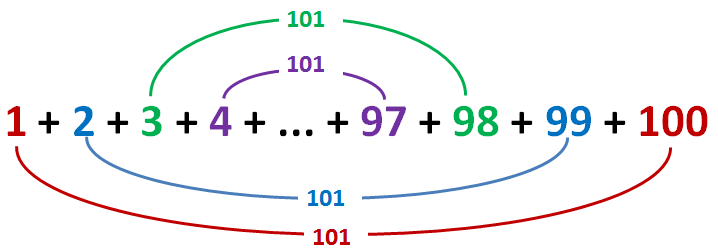
\includegraphics[width=\textwidth]{kleiner-gauss}
    \end{column}
  \end{columns}
\end{frame}


\section{Wo ist Waldo?}

\begin{frame}{Wo ist Waldo?}
  \centering
  
\includegraphics[height=0.8\textheight]{waldo}
\end{frame}


\section{Ali Baba}

\begin{frame}{Ali Baba}
  \centering
  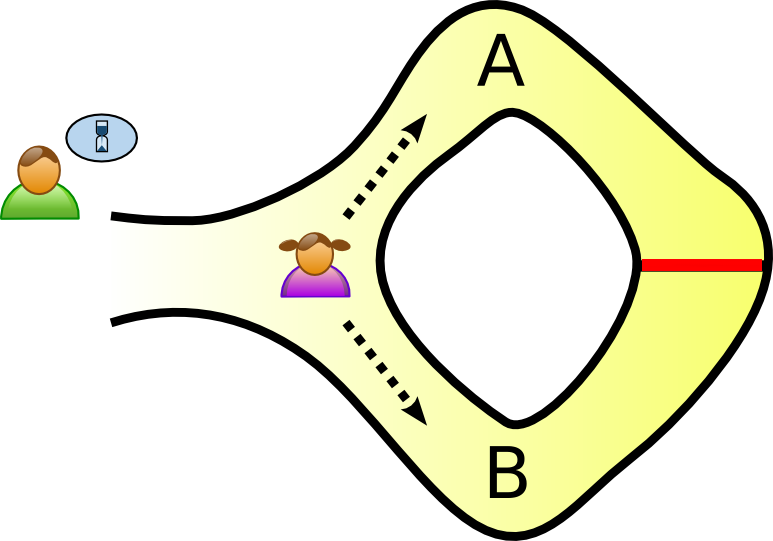
\includegraphics[height=0.8\textheight]{alibaba1}
\end{frame}


\appendix

\begin{frame}{Mathecamp}
  \centering
  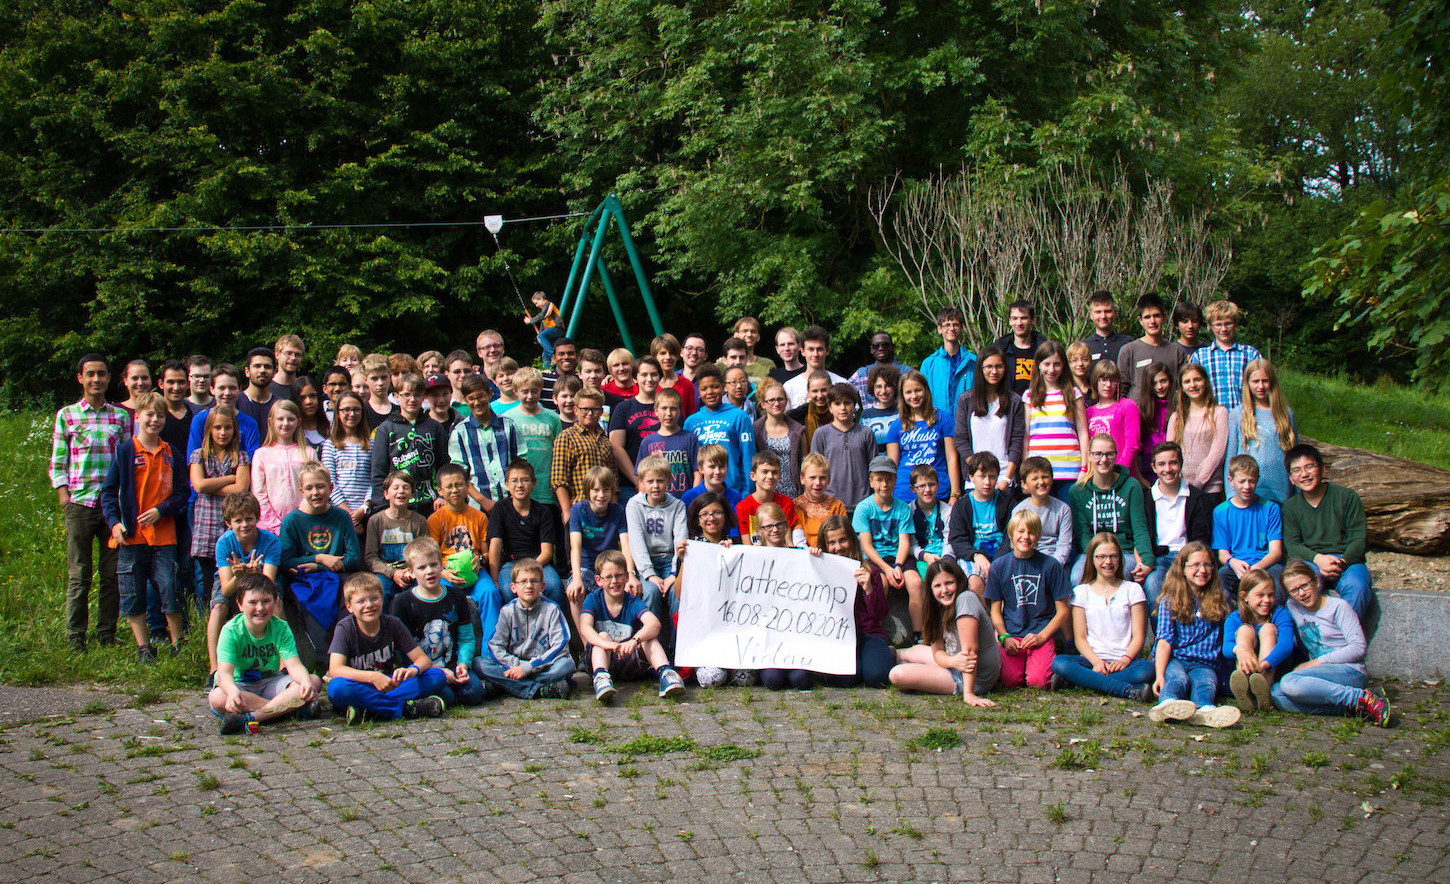
\includegraphics[width=0.9\textwidth]{mathecamp-gruppenfoto}
  \medskip

  \redheart{} 18. bis 26. August in Violau \redheart{}
\end{frame}

\end{document}
